\documentclass[11pt]{article}
\usepackage[margin=1in]{geometry}
\usepackage{graphicx}
\usepackage{booktabs}
\usepackage{siunitx}
\usepackage{caption}
\usepackage{subcaption}
\usepackage{float}
\usepackage{hyperref}
\sisetup{detect-all}
\graphicspath{{../exp/}}


\title{Shifter}
\author{Eric Xin, Shi Tao}
\date{November 18, 2026}

\begin{document}
\maketitle

%--------------------------------------------------------------------------
\section{Objective}
Design an 8-bit shifter (\texttt{Shifter\_8bit\_sized}) in the TSMC 65\,nm GP
process, verify that layout matches schematic, and characterize its
transition time (slew), propagation delay and power in transient simulation.

%--------------------------------------------------------------------------
\section{Design}
The shifter is a three-stage logarithmic shifter. Stage $k$ ($k=0,1,2$) is a
row of eight 2:1 multiplexers controlled by select bit $S_k$, which either
passes each bit through or takes the bit $2^k$ positions away, so the three
stages together realize any shift amount $0$--$7$. The shifter performs a
logical right shift, $Y_i = A_{i+S}$ with zeros shifted into the vacated
upper bits, where $S = 4S_2 + 2S_1 + S_0$. Complementary selects
$S_k$/$\overline{S_k}$ are provided at the cell boundary.

Each multiplexer is built from two CMOS transmission gates (TGs) whose NMOS
and PMOS have equal width and are controlled by the complementary selects
$S_k$/$\overline{S_k}$ (Fig.~\ref{fig:mux}); the three stages use
$3 \times 8 = 24$ multiplexers. Since TGs do not restore signal levels, an
inverter is placed at the input, between consecutive stages and at the output.
Each stage is then an inverter driving a TG, an effective stack of two;
without the intermediate inverters, the path from the input inverter to the
output would be a stack of four. Every inverter output fans out to two TGs:
the ``0'' input of its own bit's multiplexer and the ``1'' input of the
multiplexer $2^k$ bits below. The inverters are sized up from input to output
(\texttt{INV\_1}$\rightarrow$\texttt{INV\_4}) to drive the output load
(Section~\ref{sec:sizing}).

\begin{table}[H]
\centering
\caption{Cell hierarchy of \texttt{Shifter\_8bit\_sized} (signal path order).}
\label{tab:hier}
\begin{tabular}{llcl}
\toprule
Position & Cell & Instances & Function \\
\midrule
Input       & \texttt{INV\_1}      & 8 & input inverter \\
Stage 0     & \texttt{MUX2to1\_1}  & 8 & TG mux, shift by 1 ($S_0$) \\
            & \texttt{INV\_2}      & 8 & level restore \\
Stage 1     & \texttt{MUX2to1\_2}  & 8 & TG mux, shift by 2 ($S_1$) \\
            & \texttt{INV\_3}      & 8 & level restore \\
Stage 2     & \texttt{MUX2to1\_3}  & 8 & TG mux, shift by 4 ($S_2$) \\
Output      & \texttt{INV\_4}      & 8 & output driver \\
\midrule
\multicolumn{2}{l}{Ports} & \multicolumn{2}{l}{$A_{7:0}$, $S_{2:0}$, $\overline{S}_{2:0}$, $Y_{7:0}$, VDD, VSS} \\
\bottomrule
\end{tabular}
\end{table}

\begin{figure}[H]
\centering
\begin{subfigure}[b]{0.48\linewidth}
  \centering
  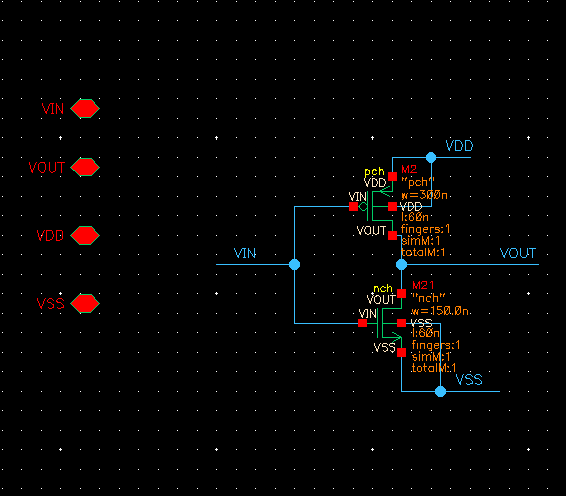
\includegraphics[width=\linewidth]{inv_std_size.png}
  \caption{Reference inverter \texttt{INV\_150n}: PMOS $W/L = 300\,\text{n}/60\,\text{n}$,
           NMOS $W/L = 150\,\text{n}/60\,\text{n}$.}
  \label{fig:inv}
\end{subfigure}\hfill
\begin{subfigure}[b]{0.48\linewidth}
  \centering
  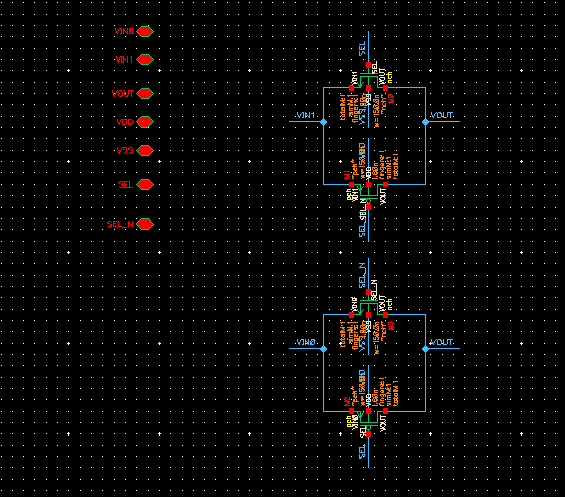
\includegraphics[width=\linewidth]{shifter_mux.png}
  \caption{2:1 multiplexer from two transmission gates
           (\texttt{VIN0}, \texttt{VIN1}, \texttt{SEL}, \texttt{SEL\_N}).}
  \label{fig:mux}
\end{subfigure}
\caption{Leaf cells.}
\end{figure}

\begin{figure}[H]
\centering
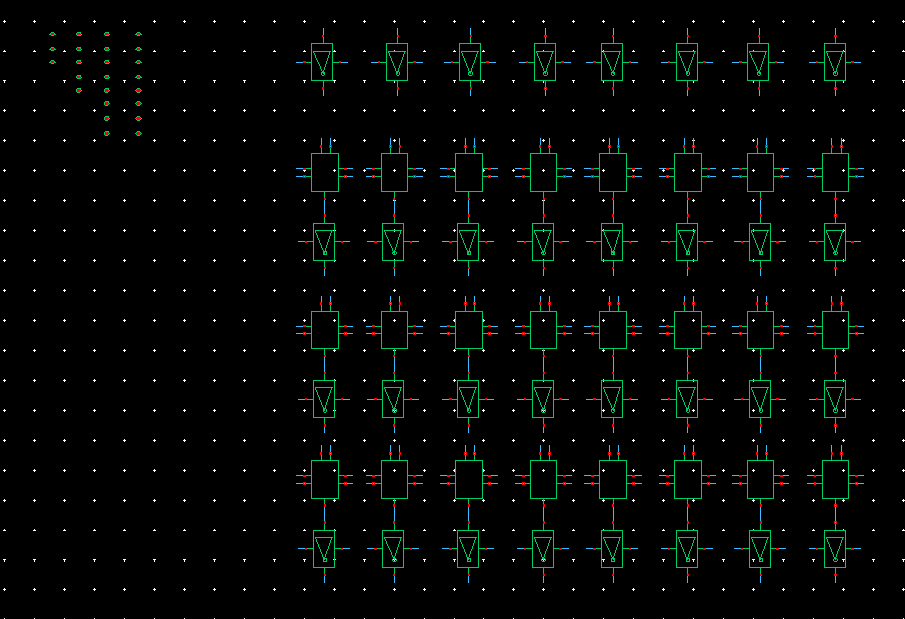
\includegraphics[width=0.8\linewidth]{shcematic.png}
\caption{Shifter schematic: input inverter row followed by three
multiplexer\,+\,inverter rows (one per shift stage).}
\label{fig:sch}
\end{figure}

\subsection{Signal polarity and zero fill}
The data path contains four inverters, so $Y$ is in phase with $A$, but the
polarity of the intermediate nodes alternates: stage~0 carries inverted
data, stage~1 true data and stage~2 inverted data. The constant shifted into
the vacated bits must represent logic~0 in each stage's polarity, so it is
tied to VDD in stage~0 (1 multiplexer), to GND in stage~1 (2 multiplexers)
and to VDD in stage~2 (4 multiplexers): five fill inputs go to VDD and two to
GND.

\subsection{Transistor sizing}
\label{sec:sizing}
The data path was sized with the method of logical effort under the
following assumptions. All widths are in units of the NMOS width of the
minimum inverter ($W_N = \SI{150}{nm}$).
\begin{itemize}
  \setlength\itemsep{0pt}
  \item Minimum inverter: $N=1$, $P=2$, input capacitance 3.
  \item A TG with $N=P=w$ has an equivalent resistance of about $R/w$ in
        both directions (Weste \& Harris approximation).
  \item Each output $Y$ drives 4 minimum inverters, a load of 12; the input
        inverter on $A$ is minimum size, so the path input capacitance is 3.
  \item $S_k$ and $\overline{S_k}$ are supplied externally, each driven by a
        $4\times$ minimum inverter whose load is accounted for by the
        external circuit.
  \item Parasitic delays are estimated with the Elmore model, with $p=1$ for
        the minimum inverter; delays are in units of $\tau$.
\end{itemize}

An inverter\,+\,TG stage needs an inverter of $N=2$, $P=4$ and a TG of
$N=P=2$ to match the drive of a unit inverter; its input capacitance is 6,
so $g = 6/3 = 2$. The TG width is set equal to the NMOS width of the
inverter that drives it. For the four-stage path,
\[
G = 2\cdot2\cdot2\cdot1 = 8,\quad B = 1,\quad H = 12/3 = 4,\quad
F = GBH = 32,\quad \hat f = F^{1/4} = 2^{5/4} \approx 2.38 .
\]
Working back from the load with $C_\text{in} = g\,C_\text{out}/\hat f$ gives
input capacitances of 5.05 (output inverter), 4.24, 3.57 and 3.00 (input
inverter). Only the inverter's input capacitance counts as $C_\text{in}$ of
an inverter\,+\,TG stage: the TG gates connect to the select lines, and the
TG diffusion capacitance is counted as parasitic delay rather than
$C_\text{out}$. Each stage is therefore $2^{1/4} \approx 1.19$ times larger
than the one before (Table~\ref{tab:sizing}).

\begin{table}[H]
\centering
\caption{Theoretical data-path sizes ($N/P$ in units of $W_N=\SI{150}{nm}$),
before rounding.}
\label{tab:sizing}
\begin{tabular}{llcc}
\toprule
Element & Cell & $N$ / $P$ & $W_N$ (nm) \\
\midrule
Input inverter ($A$)        & \texttt{INV\_1}     & 1 / 2         & 150 \\
Stage 0 TG                  & \texttt{MUX2to1\_1} & 1 / 1         & 150 \\
Inverter, stage 0$\to$1     & \texttt{INV\_2}     & 1.19 / 2.38   & 178 \\
Stage 1 TG                  & \texttt{MUX2to1\_2} & 1.19 / 1.19   & 178 \\
Inverter, stage 1$\to$2     & \texttt{INV\_3}     & 1.41 / 2.83   & 212 \\
Stage 2 TG                  & \texttt{MUX2to1\_3} & 1.41 / 1.41   & 212 \\
Output inverter             & \texttt{INV\_4}     & 1.68 / 3.36   & 252 \\
\bottomrule
\end{tabular}
\end{table}

\paragraph{Select lines.} Each multiplexer loads $S_k$ and
$\overline{S_k}$ with one NMOS and one PMOS gate of width $w$, so the eight
multiplexers present $16w$: 16, 19.0 and 22.6 on $S_0$, $S_1$ and $S_2$.
Driven by the $4\times$ inverter (input capacitance 12), the path effort is
only 1.33--1.89, so the optimum number of stages is one and the selects
connect directly to the TG gates without buffers. The estimated delays
($L/12 + 1$) are 2.3, 2.6 and 2.9\,$\tau$, far below the data path, so the
selects are not on the critical path.

\paragraph{Delay estimate.} Each inverter\,+\,TG stage has a parasitic delay
of about 5 and the output inverter 1, so $P = 16$ and the sized path delay
is $D = 4 \times 2.38 + 16 \approx 25.5\,\tau$. With all devices at minimum
size the stage efforts are 2, 2, 2 and 4, giving $D \approx 26\,\tau$, only
about 2\,\% slower. Sizing gains little here because $H$ is only 4, so the
minimum-size efforts are already nearly balanced, and because parasitic
delay, which does not depend on size, is over 60\,\% of the total. With a
load of 64 minimum inverters the effort delay would be about 70 at minimum
size versus about 19 when sized, and sizing would matter.

\subsection{Layout implementation}
The multiplexer and inverter cells use a fixed cell height. A transistor too
wide to fit in that height as a single finger is split into several parallel
fingers, which keeps the cells compact and the total area small. Multiplying
the relative sizes by \SI{150}{nm} gives widths with many decimals, while the
process requires widths on a \SI{5}{nm} grid (otherwise LVS fails), so each
finger width is rounded to the nearest multiple of \SI{5}{nm}.

\paragraph{Possible optimization.} The TGs on the fill inputs could be
replaced by single transistors that pass their constant in the strong
direction (PMOS for VDD, NMOS for GND), reducing the select-line load and the
diffusion capacitance on those nodes.

%--------------------------------------------------------------------------
\section{Verification}

\subsection{Physical verification}
The layout (Fig.~\ref{fig:layout}) was checked with Calibre nmDRC and nmLVS
v2025.1\_16.10. DRC reports no violations (Fig.~\ref{fig:drc}; the only
listed check is the informational density print), and LVS against the
schematic netlist reports \textbf{CORRECT} (Fig.~\ref{fig:lvs}).

\begin{figure}[H]
\centering
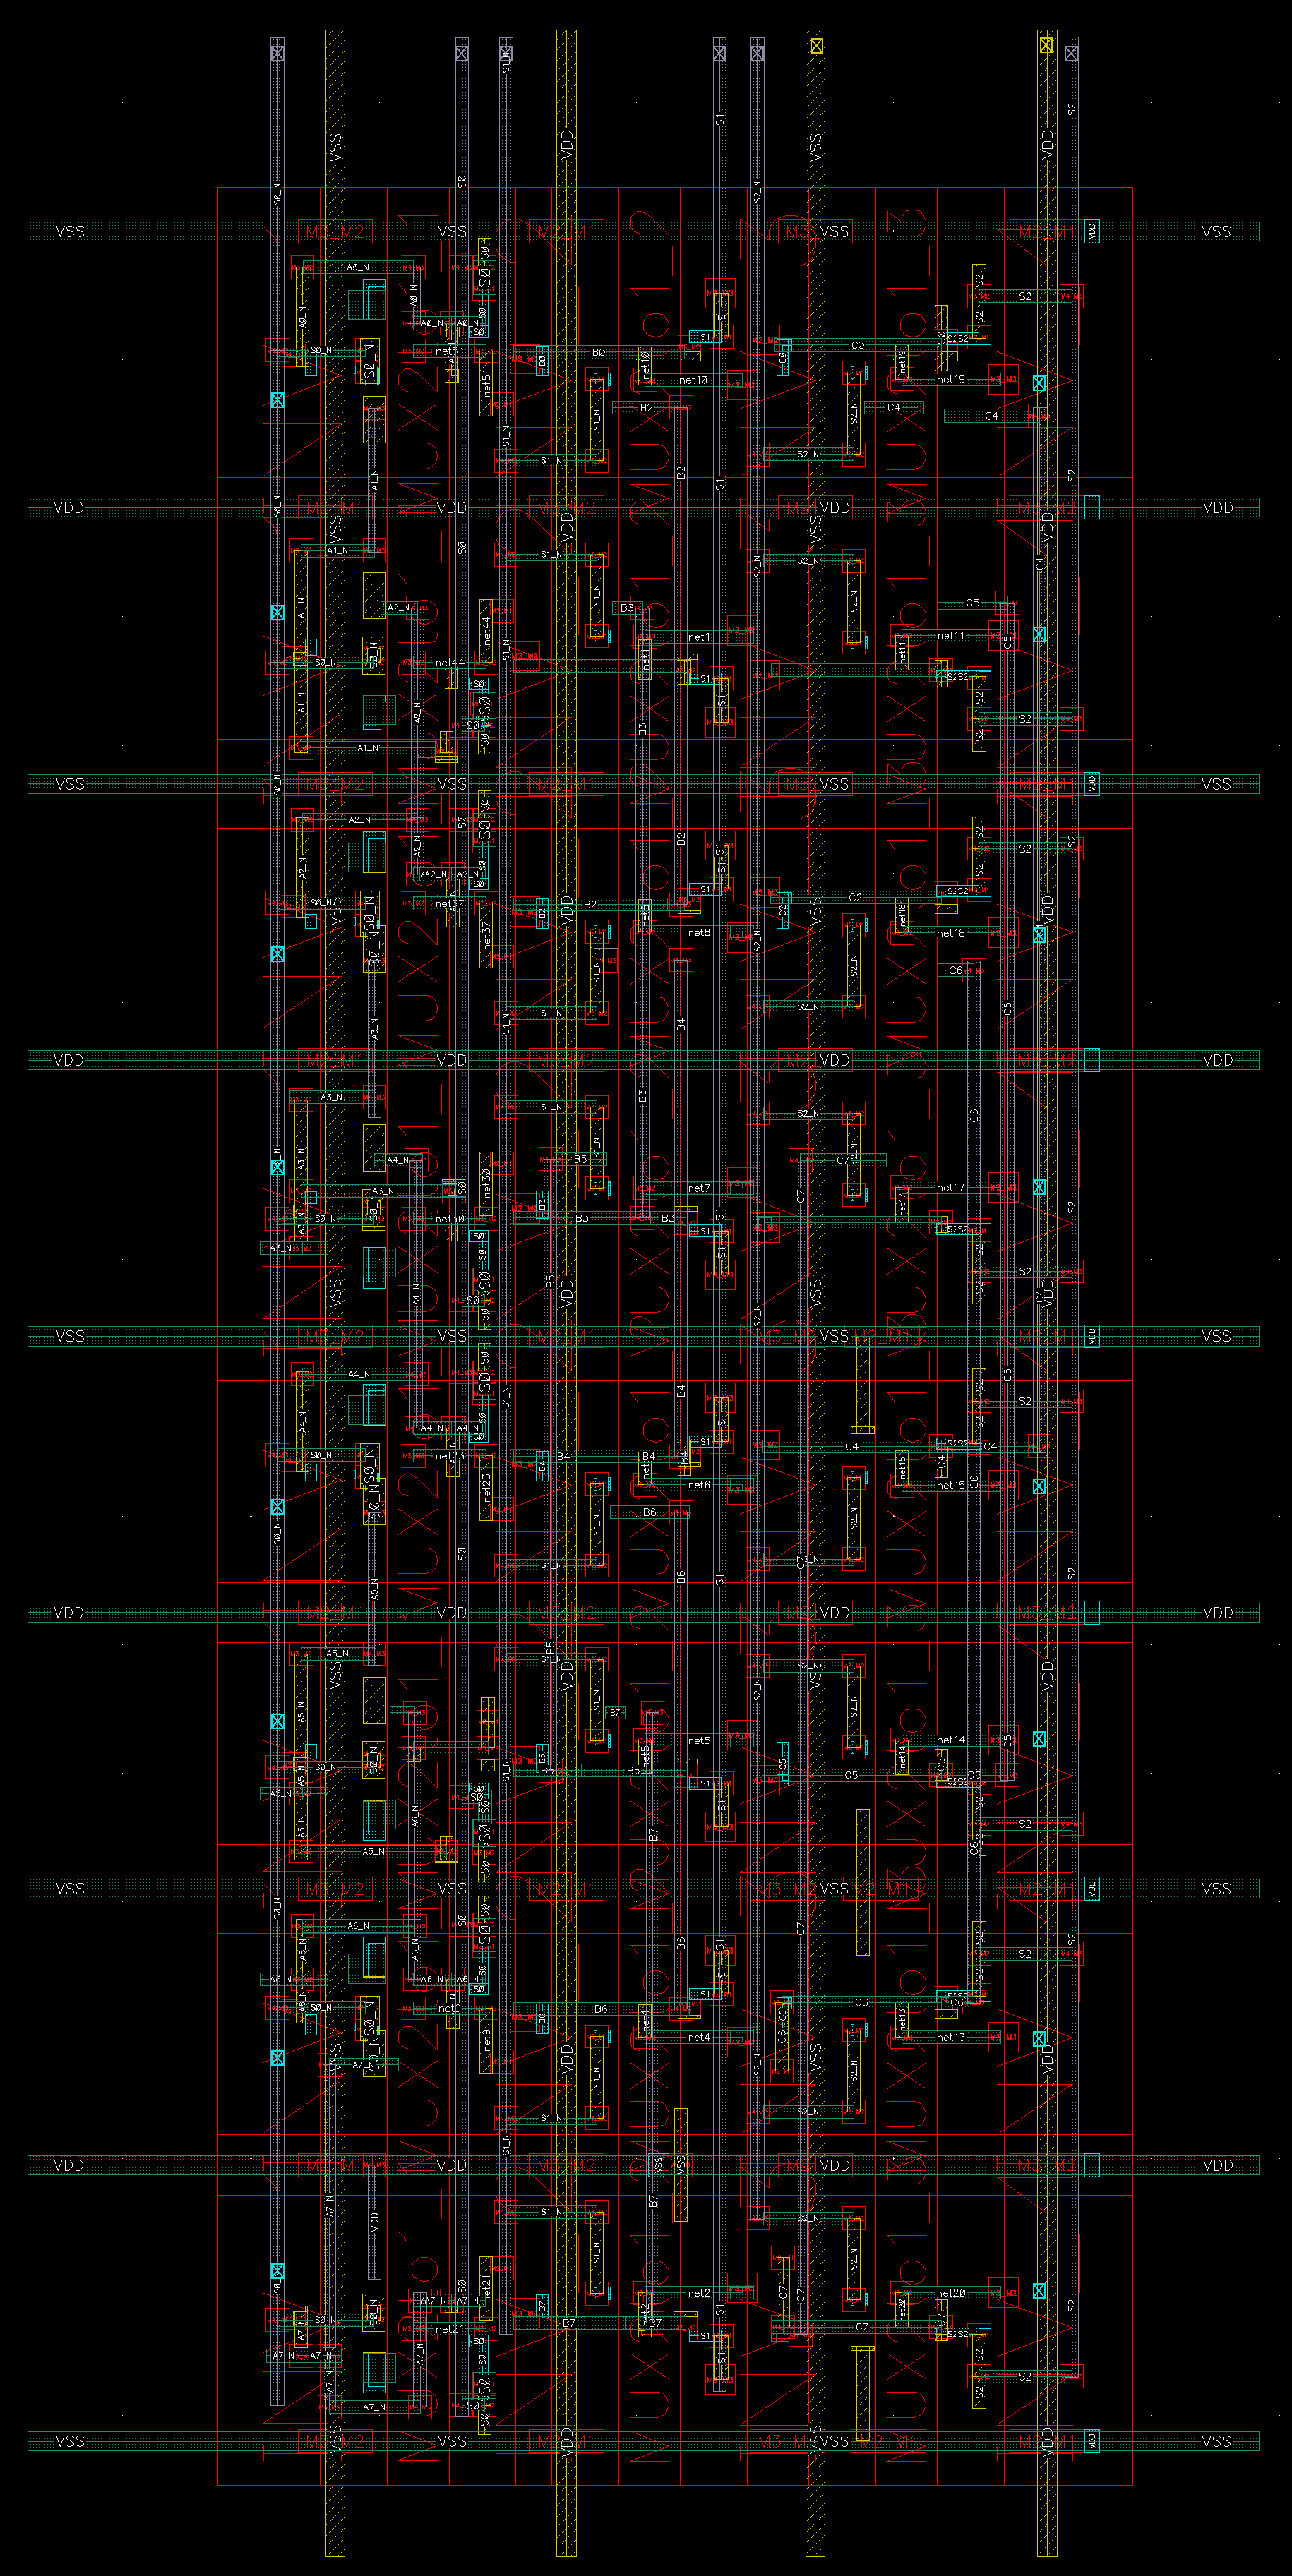
\includegraphics[height=0.72\textheight]{shifter_layout_crop.png}
\caption{Layout of \texttt{Shifter\_8bit\_sized}: eight bit rows between
alternating VDD/VSS rails, multiplexer/inverter stages in columns.}
\label{fig:layout}
\end{figure}

\begin{figure}[H]
\centering
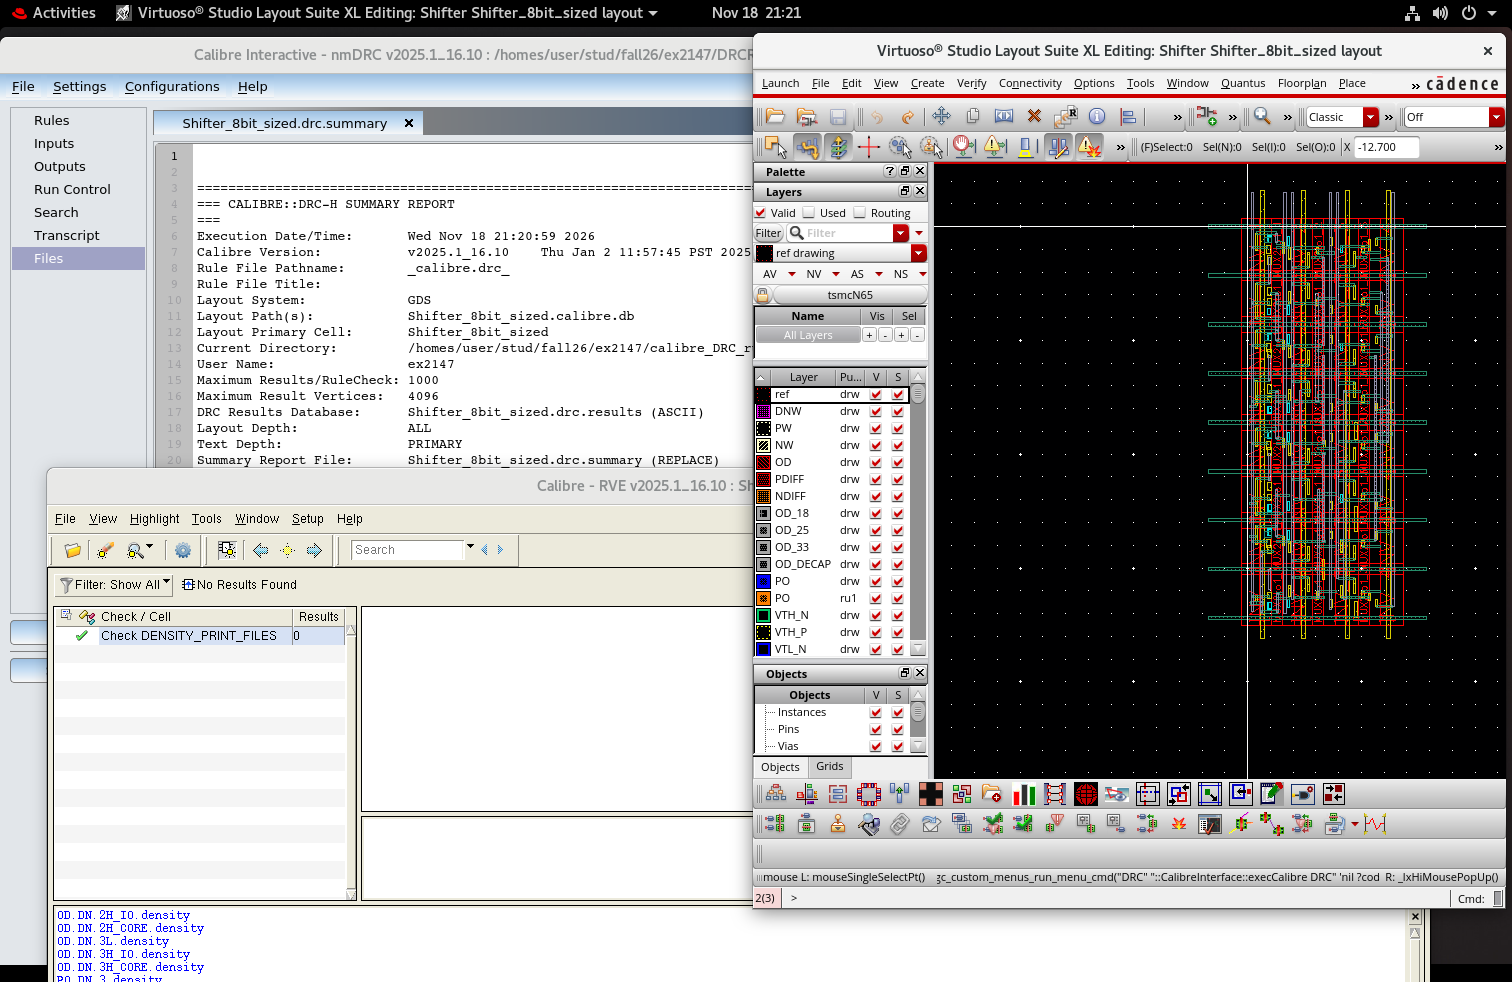
\includegraphics[width=\linewidth]{shifter_designclean.png}
\caption{Calibre DRC summary and RVE for \texttt{Shifter\_8bit\_sized}: no
rule violations.}
\label{fig:drc}
\end{figure}

\begin{figure}[H]
\centering
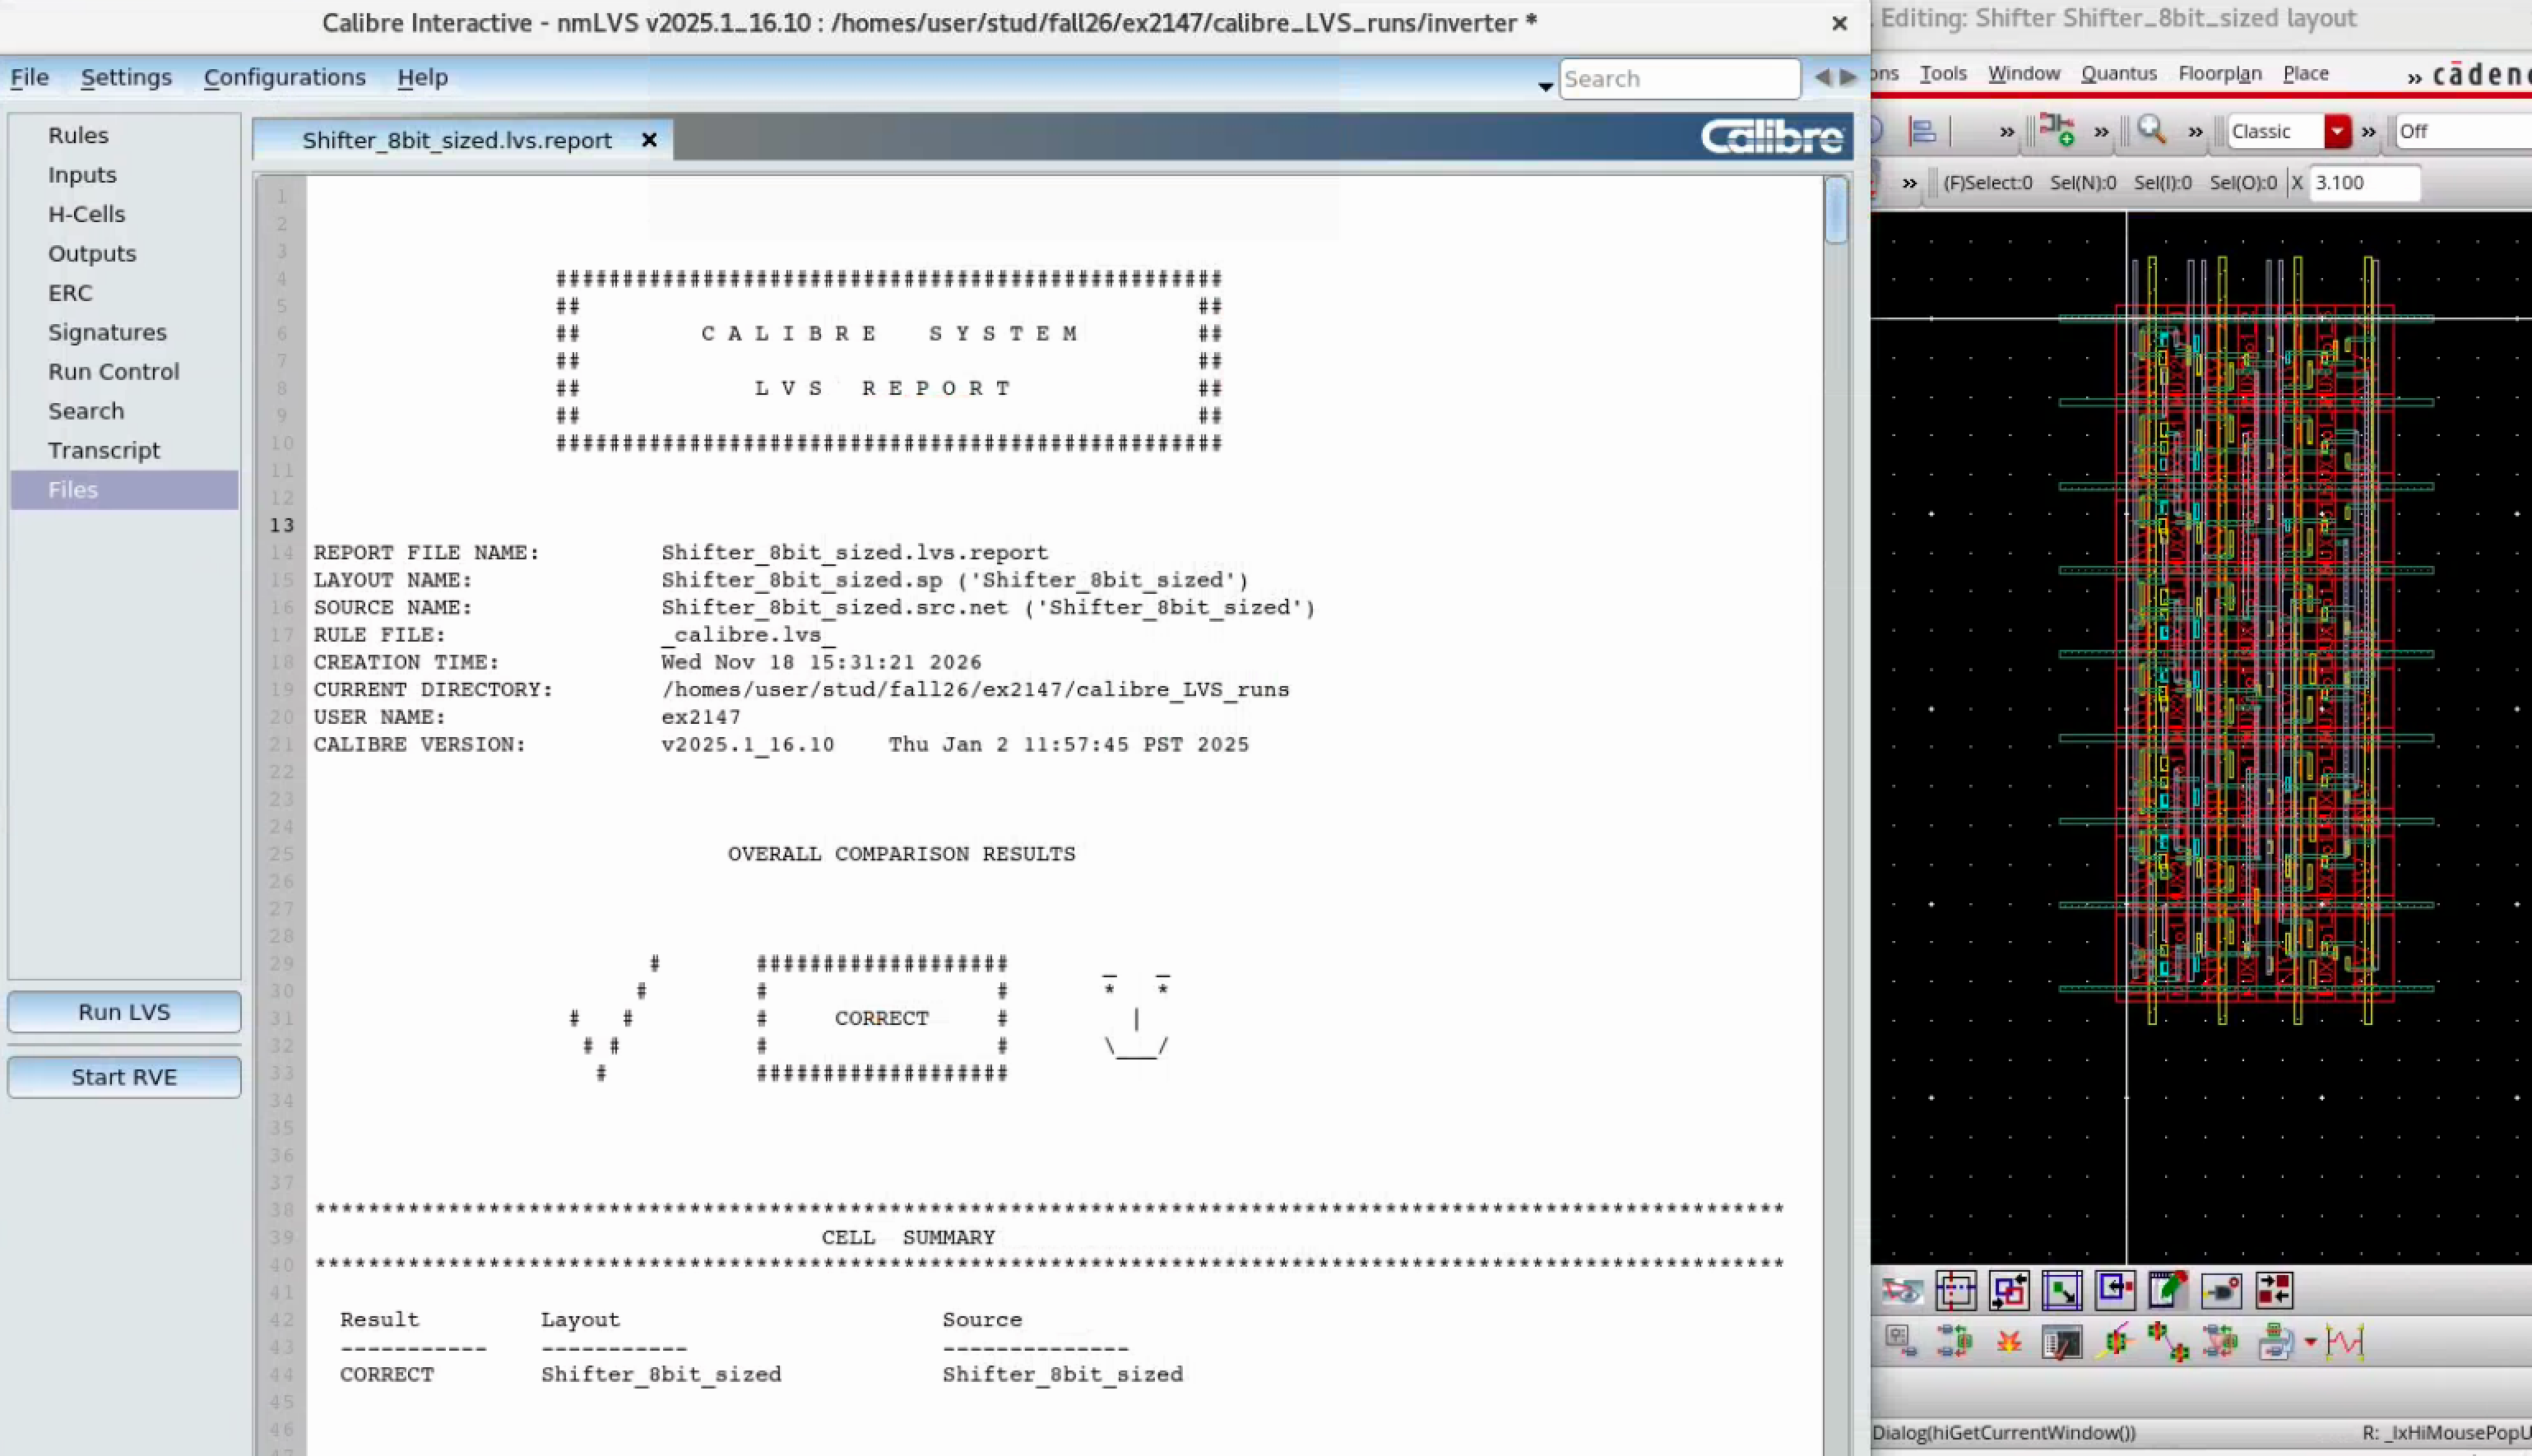
\includegraphics[width=\linewidth]{lvs_report.png}
\caption{Calibre LVS report: overall comparison result CORRECT for
\texttt{Shifter\_8bit\_sized}.}
\label{fig:lvs}
\end{figure}

\subsection{Functional verification}
The shifter was simulated at transistor level in ADE with a Verilog-A
testbench block that drives all $2^8 \times 2^3 = 2048$ combinations of $A$
and $S$ (one vector every \SI{2}{ns}), samples $Y$ at 90\,\% of each vector
period and compares it with the expected logical right shift. All 2048
vectors pass in both Spectre and UltraSim.

\begin{table}[H]
\centering
\caption{Verification summary.}
\label{tab:verif}
\begin{tabular}{lll}
\toprule
Check & Tool & Result \\
\midrule
DRC                               & Calibre nmDRC v2025.1  & clean \\
LVS (layout vs.\ schematic)       & Calibre nmLVS v2025.1  & CORRECT \\
Function, 2048 vectors            & Spectre 23.1 (APS)     & 2048/2048 pass \\
Function, 2048 vectors            & UltraSim 18.1          & 2048/2048 pass \\
\bottomrule
\end{tabular}
\end{table}

%--------------------------------------------------------------------------
\section{Characterization}

\subsection{Setup}
The same Verilog-A block measures the metrics during the simulation. It sits
in series with the shifter's VDD pin as a \SI{0}{V} ammeter, so power and
energy include only the shifter and not its loads. Each output drives four
parallel \texttt{INV\_150n} inverters (a fanout-of-4 load).

\begin{table}[H]
\centering
\caption{Simulation conditions.}
\label{tab:setup}
\begin{tabular}{ll}
\toprule
Parameter & Value \\
\midrule
Process / models      & TSMC 65\,nm GP, \texttt{crn65gplus\_2d5\_lk\_v1d0}, TT \\
Supply $V_{DD}$       & \SI{1.0}{V} \\
Temperature           & \SI{27}{\celsius} \\
Simulators            & Spectre 23.1 (APS, \texttt{errpreset=conservative}); UltraSim 18.1 \\
Analysis              & transient, \SIrange{0}{10}{\micro s} \\
Stimulus              & 2048 vectors, \SI{2}{ns} each from $t=\SI{2}{ns}$, edges \SI{25}{ps} \\
Circuit size          & 224 MOSFETs (160 shifter, 64 load), 105 nodes \\
Output load           & 4 $\times$ \texttt{INV\_150n} per output \\
Slew definition       & 10\,\%--90\,\% of $V_{DD}$, every output edge \\
Delay definition      & 50\,\% of input edge $\rightarrow$ 50\,\% of output edge \\
Power                 & $V_{DD} \times$ current into the shifter's VDD pin \\
\bottomrule
\end{tabular}
\end{table}

Because every vector changes the inputs at a known time, the delay of each
output edge is measured from the input transition of its own vector; it
covers both data ($A \rightarrow Y$) and select ($S \rightarrow Y$) paths,
over 1003 output transitions in total.

\subsection{Results}

\begin{table}[H]
\centering
\caption{Measured metrics, schematic (pre-layout), over all outputs and all
2048 vectors. Spectre is the reference; UltraSim is a fast-SPICE cross-check.}
\label{tab:results}
\begin{tabular}{l S[table-format=3.2] S[table-format=3.2] l}
\toprule
Metric & {Spectre} & {UltraSim} & Unit \\
\midrule
Rise slew, max                    & 20.63  & 24.39  & ps \\
Fall slew, max                    & 50.31  & 43.80  & ps \\
Delay $t_{pd}$, max               & 74.73  & 72.12  & ps \\
Delay $t_{pd}$, average           & 69.97  & 66.52  & ps \\
Output transitions measured       & {1003} & {1003} & \\
\midrule
Average power (\SI{10}{\micro s}) & 1.124  & 1.029  & \si{\micro W} \\
Peak power                        & 706.37 & 667.43 & \si{\micro W} \\
Total energy                      & 11.24  & 10.29  & pJ \\
Energy per output transition      & 11.20  & 10.26  & fJ \\
Energy per vector                 & 5.49   & 5.03   & fJ \\
\bottomrule
\end{tabular}
\end{table}

The worst-case propagation delay is \SI{74.7}{ps} with an average of
\SI{70.0}{ps}. Output falling edges are slower than rising edges
(\SI{50.3}{ps} versus \SI{20.6}{ps} worst-case slew), which suggests the
output inverter's pull-down is the weaker side for this load. UltraSim agrees with
Spectre to within about 20\,\% on slew and 5\,\% on delay, as expected for a
fast-SPICE engine.

\begin{table}[H]
\centering
\caption{Per-output timing, UltraSim (schematic), all 2048 vectors. Times in ps.}
\label{tab:perout}
\begin{tabular}{lrrrrrrr}
\toprule
 & \multicolumn{2}{c}{Rise slew} & \multicolumn{2}{c}{Fall slew} & \multicolumn{2}{c}{Delay $t_{pd}$} & \\
\cmidrule(lr){2-3}\cmidrule(lr){4-5}\cmidrule(lr){6-7}
Output & max & avg & max & avg & max & avg & Edges \\
\midrule
$Y_0$ & 24.39 & 22.74 & 23.68 & 22.60 & 71.81 & 65.87 & 509 \\
$Y_1$ & 23.17 & 22.19 & 43.80 & 22.58 & 71.79 & 66.60 & 254 \\
$Y_2$ & 22.92 & 21.54 & 43.34 & 22.28 & 71.63 & 67.97 & 126 \\
$Y_3$ & 22.72 & 21.47 & 23.66 & 21.99 & 70.50 & 67.53 & 62 \\
$Y_4$ & 22.93 & 21.20 & 23.04 & 21.77 & 72.12 & 68.62 & 30 \\
$Y_5$ & 22.38 & 21.06 & 23.17 & 21.99 & 72.02 & 67.33 & 14 \\
$Y_6$ & 21.07 & 20.79 & 22.57 & 21.99 & 71.85 & 64.47 & 6 \\
$Y_7$ & 20.82 & 20.82 & 21.93 & 21.93 & 69.11 & 64.63 & 2 \\
\midrule
All & 24.39 & 22.28 & 43.80 & 22.48 & 72.12 & 66.52 & 1003 \\
\bottomrule
\end{tabular}
\end{table}

The edge count falls by roughly half per bit from $Y_0$ (509) to $Y_7$ (2):
under a right shift the upper outputs receive more shifted-in zeros, and
$Y_7$ follows $A_7$ only when $S=0$. Average slews are uniform at
21--23\,ps on every output; the worst-case fall slew of about 44\,ps occurs
only on a few edges of $Y_1$ and $Y_2$, while their average fall slew stays
at 22\,ps.

The average power is quoted over the full \SI{10}{\micro s} window, of which
the vector sweep occupies the first \SI{4.1}{\micro s}; the energy per output
transition (\SI{11.2}{fJ}) and per vector (\SI{5.5}{fJ}) are the more useful
figures, since they do not depend on the window length.

%--------------------------------------------------------------------------
\section{Pre- versus post-layout}
Parasitics were extracted with Calibre (R\,+\,C\,+\,coupling C) into the
\texttt{calibre} view, which replaces the schematic of the shifter in the same
testbench (view list \texttt{calibre} before \texttt{schematic}). The
extracted netlist grows from 105 to 5428 nodes and adds 5479 resistors and
16\,047 capacitors to the 224 transistors. It was simulated in Spectre 23.1
(APS, \texttt{errpreset=moderate}; \SI{26.6}{min} wall time, 166\,035 time
steps), and the extracted shifter still passes all 2048 vectors.

\begin{table}[H]
\centering
\caption{Schematic versus extracted layout (Spectre, all outputs, all 2048 vectors).}
\label{tab:prepost}
\begin{tabular}{l S[table-format=3.2] S[table-format=3.2] r}
\toprule
Metric & {Schematic} & {Post-layout} & Change \\
\midrule
Rise slew, max (ps)                 & 20.63  & 47.02  & $+128\,\%$ \\
Fall slew, max (ps)                 & 50.31  & 119.88 & $+138\,\%$ \\
Delay $t_{pd}$, max (ps)            & 74.73  & 180.94 & $+142\,\%$ \\
Delay $t_{pd}$, avg (ps)            & 69.97  & 142.22 & $+103\,\%$ \\
\midrule
Average power, \SI{10}{\micro s} (\si{\micro W}) & 1.124 & 1.896 & $+69\,\%$ \\
Peak power (\si{\micro W})          & 706.37 & 811.19 & $+15\,\%$ \\
Total energy (pJ)                   & 11.24  & 18.96  & $+69\,\%$ \\
Energy per output transition (fJ)   & 11.20  & 18.90  & $+69\,\%$ \\
Energy per vector (fJ)              & 5.49   & 9.26   & $+69\,\%$ \\
\midrule
Function (2048 vectors)             & {pass} & {pass} & \\
\bottomrule
\end{tabular}
\end{table}

Layout parasitics roughly double the propagation delay (average
\SI{70.0}{ps} $\rightarrow$ \SI{142.2}{ps}, worst case \SI{74.7}{ps}
$\rightarrow$ \SI{180.9}{ps}) and increase the worst-case output slews by a
factor of 2.3--2.4. The energy per transition rises by 69\,\%, which is the
extra wiring capacitance charged on every switching event, while the peak
power rises only 15\,\%, since the added RC spreads the switching current
over a longer time. The select lines run vertically across all eight bit
rows and each drives eight transmission gates, so their wire capacitance is
a likely large contributor; reducing it (wider spacing, a select buffer per
stage, or shorter routes) is the main lever for recovering speed.

\begin{table}[H]
\centering
\caption{Per-output timing, Spectre (post-layout), all 2048 vectors. Times in ps.}
\label{tab:perout_pex}
\begin{tabular}{lrrrrrrr}
\toprule
 & \multicolumn{2}{c}{Rise slew} & \multicolumn{2}{c}{Fall slew} & \multicolumn{2}{c}{Delay $t_{pd}$} & \\
\cmidrule(lr){2-3}\cmidrule(lr){4-5}\cmidrule(lr){6-7}
Output & max & avg & max & avg & max & avg & Edges \\
\midrule
$Y_0$ & 46.65 & 44.01 & 47.38 & 36.73 & 180.55 & 138.09 & 509 \\
$Y_1$ & 47.02 & 43.75 & 119.88 & 37.24 & 176.18 & 141.80 & 254 \\
$Y_2$ & 46.50 & 44.01 & 115.48 & 37.70 & 172.37 & 148.76 & 126 \\
$Y_3$ & 46.10 & 43.85 & 40.47 & 36.38 & 167.26 & 148.22 & 62 \\
$Y_4$ & 46.68 & 46.53 & 46.04 & 42.72 & 180.94 & 164.47 & 30 \\
$Y_5$ & 47.02 & 46.92 & 44.30 & 41.83 & 175.78 & 161.65 & 14 \\
$Y_6$ & 46.43 & 46.34 & 40.33 & 39.99 & 171.84 & 151.10 & 6 \\
$Y_7$ & 45.97 & 45.97 & 40.90 & 40.90 & 165.95 & 149.43 & 2 \\
\midrule
All & 47.02 & 44.07 & 119.88 & 37.24 & 180.94 & 142.22 & 1003 \\
\bottomrule
\end{tabular}
\end{table}

Per output (Table~\ref{tab:perout_pex}), the average rise and fall slews stay
uniform at 36--47\,ps, and as in the schematic the worst-case fall slew
(about 115--120\,ps) occurs only on a few edges of $Y_1$ and $Y_2$. The
upper outputs $Y_4$--$Y_7$ have a higher average delay (149--164\,ps) than
$Y_0$--$Y_3$ (138--149\,ps), but they switch on far fewer edges.
Figure~\ref{fig:wave_pex} shows the extracted shifter's waveforms around one
vector boundary.

\begin{figure}[H]
\centering
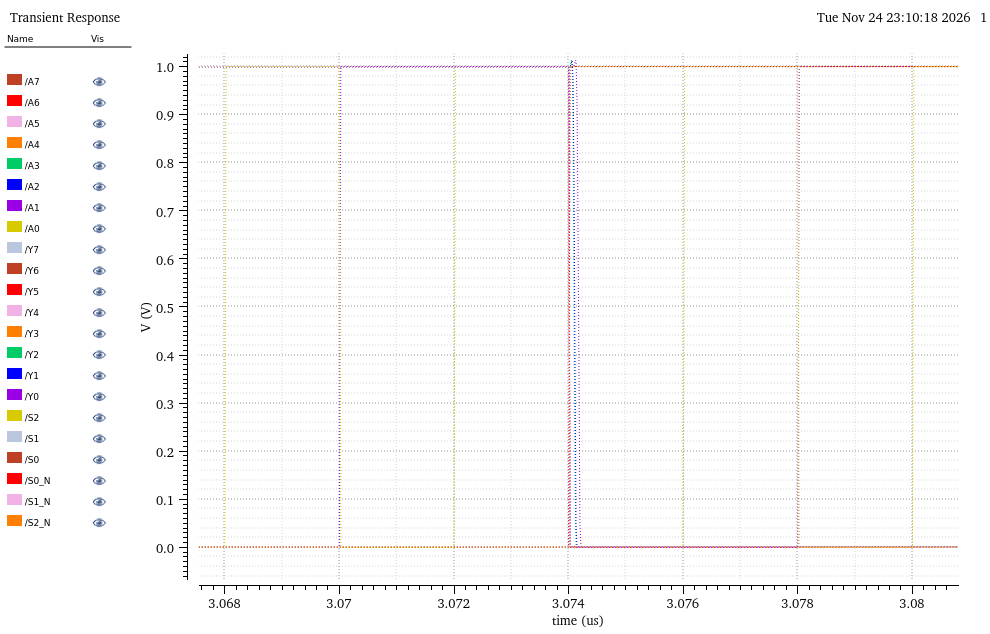
\includegraphics[width=\linewidth]{shifter_wave_pex.png}
\caption{Post-layout transient waveforms of all inputs and outputs around the
vector boundary at $t = \SI{3.074}{\micro s}$ (Spectre, extracted view).}
\label{fig:wave_pex}
\end{figure}

The schematic run used \texttt{errpreset=conservative} and the post-layout run
\texttt{moderate}. An earlier post-layout run with \texttt{liberal} gave
results within 6\,\% of the \texttt{moderate} run, so the preset accounts for
only a small part of the differences in Table~\ref{tab:prepost}.

%--------------------------------------------------------------------------
\section{Conclusion}
The 8-bit logarithmic right shifter was implemented with transmission-gate
multiplexers and progressively sized restoring inverters. The layout is DRC-
and LVS-clean, and all 2048 input/shift combinations produce the correct
output in transistor-level simulation both before and after parasitic
extraction. At \SI{1.0}{V}, TT, \SI{27}{\celsius} with a fanout-of-4 load,
the schematic achieves a worst-case delay of \SI{74.7}{ps} and
\SI{11.2}{fJ} per output transition; with extracted parasitics the
worst-case delay becomes \SI{180.9}{ps} (average \SI{142.2}{ps}), the
worst-case slews \SI{47.0}{ps} rising and \SI{119.9}{ps} falling, and the
energy \SI{18.9}{fJ} per output transition. Wiring parasitics therefore
dominate the delay of the laid-out shifter.

\end{document}
